%\chapter{DATABASE STRESS TEST}
\chapter{Database Stress Test}
\label{Database Stress Test}

%%%%%%%%%%%%%%%%%%%%%%%%%%%%%%%%%%%%%%%%%%%%%%%%%%%%%%%%%%%%%
\section{Database Stress Test}
\label{Database Stress Test}

The motivation behind this analysis was to perform quality checks of the analyzer and database. In order to do such an analysis, a dataset of N$\rightarrow\Delta$ measurement from Run 1, slug 3 and 4 was chosen for its strange behavior. This section will focus on different quality checks performed on the dataset. 



\begin{singlespace}
\begin{figure}[!h]
	\begin{center}
	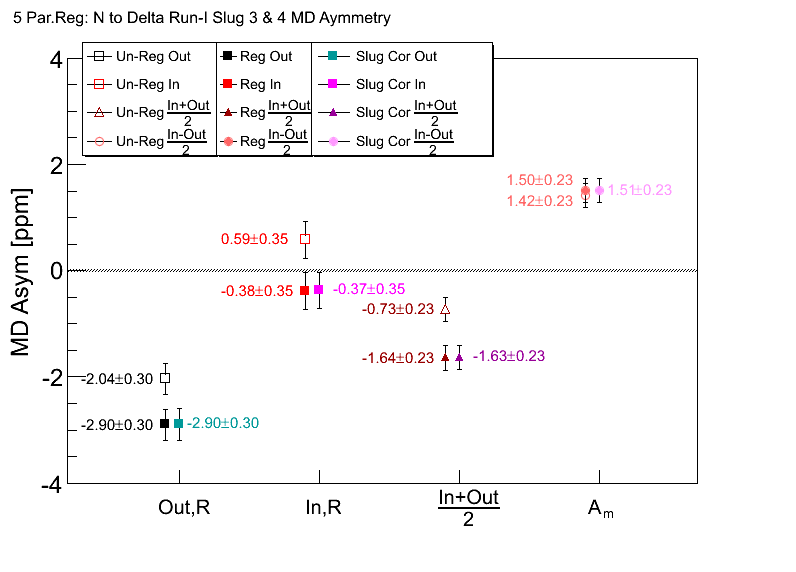
\includegraphics[width=15.0cm]{figures/n2DeltaMDSummaryPlotReg5}
	\end{center}
	\caption
%	[Main detector asymmetries for PV e-p scattering in N$\rightarrow\Delta$ dataset from Run 1 pass 4b database for slugs 3 and 4.]	
	{Main detector asymmetries for PV e-p scattering in N$\rightarrow\Delta$ dataset from Run 1 pass 4b database for slugs 3 and 4.}
	\label{fig:n2DeltaMDSummaryPlotReg5}
\end{figure}
\end{singlespace}


\subsection{Database Stress Test}
\label{Database Stress Test}

%The main detector asymmetry from Run 1 for Pass 3 5 parameter regression
%
%The regression stress test was performed on Run 1 slugs 3 and 4 datasets using pass 3 database. These are the parity violating electron-proton scattering asymmetries in the N$\rightarrow\Delta$ region.
%A closer look revealed a discrepancy between runlet numbers between un-regressed and regressed asymmetries in the database for pass 3, which was then fixed during next pass of the data analysis. 

The regression stress test was performed on the parity violating electron-proton scattering in N$\rightarrow\Delta$ region dataset from Run 1 pass 3 database for slugs 3 and 4. A closer look revealed a discrepancy between runlet numbers between un-regressed and regressed asymmetries in the database for pass 3, which was then fixed during the pass 4b. 
The weighted, un-weighted octant averaged asymmetries, and MDall asymmetries were similar. The asymmetries averaged over runlet yielded a different asymmetry compared to run averaged asymmetry. The different noise suppression in runlet and run level averaging might have created this discrepancy. 
The un-regressed IHWP-IN and correction are significantly different from this analysis, compared to an independent analysis by J. Leacock~\cite{leacock_qweak}.
The regressed MD all asymmetries in Run 1 pass4b database were consistent with~\cite{leacock_qweak}.
The regression did not improve $\chi^{2}$/DOF or probability, but improved the main detector asymmetry widths by few ppm.
Normalizing the asymmetry width with beam current didn't improve the result.
The regression also helped to remove the dipole.
The $\sim$7$\sigma$ (IN+OUT)/2 problem persists in pass4b 5 parameter regression for the dataset.
The slug averaged sensitivities give similar results.
The sensitivity vs octant looks nice.


\begin{singlespace}
\begin{figure}[!h]
	\begin{center}
	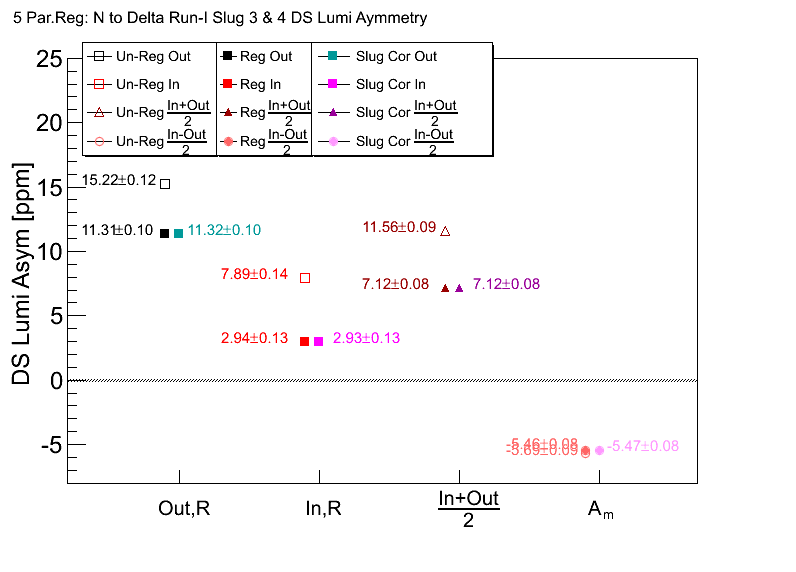
\includegraphics[width=15.0cm]{figures/n2DeltaDSLumiSummaryPlotReg5}
	\end{center}
	\caption
%	[The downstream luminosity monitor asymmetries for PV e-p scattering in N$\rightarrow\Delta$ dataset from Run 1 pass 4b database for slugs 3 and 4.]	
	{The downstream luminosity monitor asymmetries for PV e-p scattering in N$\rightarrow\Delta$ dataset from Run 1 pass 4b database for slugs 3 and 4.}
	\label{fig:n2DeltaDSLumiSummaryPlotReg5}
\end{figure}
\end{singlespace}



The same analysis was performed on DS Lumi. 
The slug average sensitivities give similar answer within $\sim$8~ppb level. 
The DS Lumi sensitivities are fairly stable but high compared to main detector. 
The  slug averaged sensitivity reduce the noise but don't improve as main detector. 
The regression improve widths by ~ 28 ppm. 
The octant averaged asymmetries didn't match DS lumi sum. 
The normalized octant yields are different. Problem found in the DS Lumi sum calculation. 
The regression didn't remove dipole completely and the dipole was too big to be transverse. 
Some significant slopes remaining after regression in few cases. 
The charge sensitivity was ~20\%. 

\begin{singlespace}
\begin{figure}[!h]
	\begin{center}
	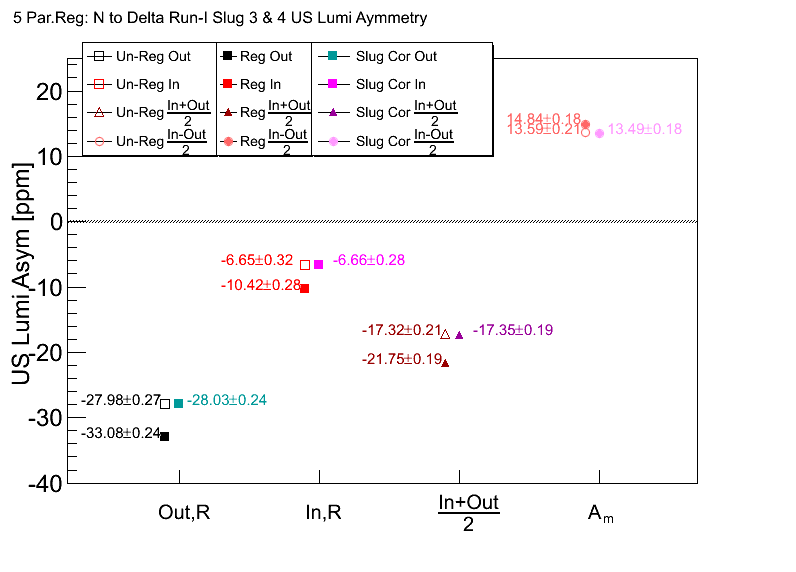
\includegraphics[width=15.0cm]{figures/n2DeltaUSLumiSummaryPlotReg5}
	\end{center}
	\caption
%	[The upstream luminosity monitor asymmetries for PV e-p scattering in N$\rightarrow\Delta$ dataset from Run 1 pass 4b database for slugs 3 and 4.]	
	{The upstream luminosity monitor asymmetries for PV e-p scattering in N$\rightarrow\Delta$ dataset from Run 1 pass 4b database for slugs 3 and 4.}
	\label{fig:n2DeltaUSLumiSummaryPlotReg5}
\end{figure}
\end{singlespace}


%Pass3:
%
%Are weighted and un-weighted octant averages similar? Yes.
%
%Are un-weighted octant averages same as MDall asymmetries? Yes.
%
%When asymmetries were averaged over runlet-by-runlet gives a somewhat different picture of the effect of regressions compared to when averaged over run-by-run.
%
%The asymmetries for IHWP-OUT state match J. Leacock's~\cite{leacock_qweak} but IHWP-IN asymmetries don't match.
%
%Un-regressed IHWP-IN and correction are significantly different for this analysis compared to John's result. 
%Both un-regressed IHWP-IN and correction are significantly different. Cuts?
%
%Regressed asymmetry vs main detector octant for IHWP-IN state seems to show large dipole like behavior. 
%
%The (In+Out)/2 and (In-Out)/2 results mirror the IHWP-IN results.
%
%
%Pass4b:
%
%Regressed MD all asymmetries in Run 1 pass4b database is consistent.
%
%
%What happened with IN+OUT problem in pass4b 5 parameter scheme.
%How slug averaged sensitivities compared to standard database.
%A look at various ways to QC regression
%
%
%Regression don't improve $\chi^{2}$/DOF or Probability. May be run-by-run regression
%will give us a better picture!
%
%Regression improve $\chi^{2}$/DOF or Probability for IN but get worse for OUT.
%
%Regression improve widths by few ppm.
%
%Normalizing width with beam current didn't help.
%
%Regression remove dipole
%
%
%$\sim$7$\sigma$ IN+OUT problem persists in pass4b 5 parameter scheme for Run 1
%N$\rightarrow\Delta$ slug 3 and 4 data set.
%
%Slug averaged sensitivities give similar results.
%
%Looked at various ways to QC regression:
%- What works: dipoles get removed, asymmetry widths smaller,
%sensitivity vs octant looks nice.
%- What doesn’t: $\chi^{2}$/DOF for constant fit to asymmetry vs run(let), MD asymmetry width don't improve by normalizing with sqrt of beam current.
%
%
%
%
%
%DS Lumi:
%
%Slug average sensitivities give similar answer within $\sim$8~ppb level
%
%Sensitivities are fairly stable but high compared to MD.
%
%Slug averaged sensitivity reduce noise but don't improve as MD
%
%Regression improve widths by ~ 28 ppm
%
%Normalizing width with beam current didn't help.
%
%Octant averaged asymmetries don't match DS lumi sum! Normalized octant yields be that different ?
%
%Normalized octant yields are different.
%
%Octant averaged asymmetries don't match DS lumi sum. Normalized octant yields are different !
%
%Regression don't remove dipole completely. Too big to be transverse !
%
%Octant-by-octant sensitivities look reasonable.
%
%Some significant slopes remaining in few cases.
%
%Charge sensitivity is ~20\%.
%
%
%Due to high DS Lumi sensitivity, very large false asymmetries in un-regressed O(10) ppm.
%
%Regression moved asymmetries for IN, OUT, and (IN+OUT)/2 in correct direction by about 4 ppm. (IN-OUT)/2 remains frozen near -5ppm.
%
%Octant averaged asymmetries don't match DS Lumi sum by factors up to 3.
%
%Can the normalized octant yields be that different ? Yes. Need to revisit DS
%Lumi sum calculation !
%
%Regression removed $\sim$80\% of dipole in octant plot.
%
%Some significant slopes remaining after regression in few cases.
%
%Charge sensitivity is large ~20\%.

%The second dataset's regressed systematic zero check, (IN + OUT)=2, was an unacceptably
%large 7$\sigma$ from zero. This dataset's quality can be seen in Figure 6.2 
%
%Notice the beam position parameters are 500 nm and the beam angle parameters are two
%orders of magnitude larger than in the initial dataset in Table 6.2. The energy variable is an
%order of magnitude larger than in the initial dataset.
%
%The process to determine the cause of the (IN+OUT)/2 = 0 check will now be discussed.
%Initially, the regression looked to be correcting with the wrong sign. This was dismissed
%as the cause after observing the complete removal of correlations between the measured
%asymmetry and the regression variables in Figures 6.3 and 6.4.
%
%Next, the linearity of the main detector bars was examined to insure each bar measured a
%similar nonlinearity. After standard regression (std) the measured asymmetry was plotted
%against the charge asymmetry variable. Standard regression does not include the charge
%asymmetry as a regression variable. The observed nonlinearities were consistent among bars
%and similar to those observed during normal production (-1.7 ppm/ppm). The nonlinearity
%did not appear to be the cause of the (IN+OUT)/2 6= 0 issue. Figure 6.7 shows the agreement
%between the main detector bar measured asymmetry. - Leacock




